% !TEX encoding = UTF-8 Unicode 

\section{Mobile development approaches}

The definition of mobile development can be interpreted in a variety of ways. It can be seen as a broad process of implementing a mobile application, starting with planning and designing and finishing with testing, releasing and maintaining. A more software-oriented definition is that mobile development simply refers to implementing an application for mobile devices by coding it using a selected technology stack \cite{microsoft_mobile_development}. In this thesis, the latter definition is assumed.

Mobile development can become a complex task considering the variety of devices and platforms existing in the market. There are many different approaches available and in order to choose one over another the mobile application requirements should be taken into account as well as target platforms and devices, development and time costs \cite{velvetech_mobile_dev_approaches}.

In this chapter, there are presented selected popular approaches to mobile application development. Each of them is described mainly in the context of architecture, technology stack and tools, platforms supported and possible advantages or disadvantages.

\subsection{Native mobile development}

Native mobile development encompasses building mobile applications that can only be implemented using a platform-specific programming language and deployed to a single operating system \cite{comparative_analysis_native_hybrid}. Such an approach brings with it the necessity for creating and maintaining multiple codebases and with that possibly multiple development teams \cite{approach_to_assess_performance_case_study}. The number of distinct codebases does not simply equal to the number of target platforms, as different versions of a single platform may require to be implemented independently \cite{appdynamics_mobile_app_performance}. Hence, development costs are high from the viewpoint of financing and time.

Native mobile applications are closely integrated with the operating system through using target platform's components \cite{comparison_perf_looks_flutter_native,comp_analysis_hybrid_frameworks} and most recent features \cite{eval_rn_flutter}. For that reason, at times they can be referred to as "embedded" 
 \cite{cross_platform_development_study_rn_flutter} and in theory should provide the maximal performance. Furthermore, because native apps are developed according to the operating system's guidelines, such as Material design system for Android and Cupertino for iOS, they are naturally easy to use for users accustomed to that specific platform.

Since almost a decade, the mobile operating system market has been dominated by Android together with iOS, reaching 99,3\% in March 2023, as shown in Figure \ref{fig:mobile_os_market}. For this reason, in the context of this thesis only the above-mentioned operating systems are being taken into consideration.

\begin{figure}[h]
  \centering
  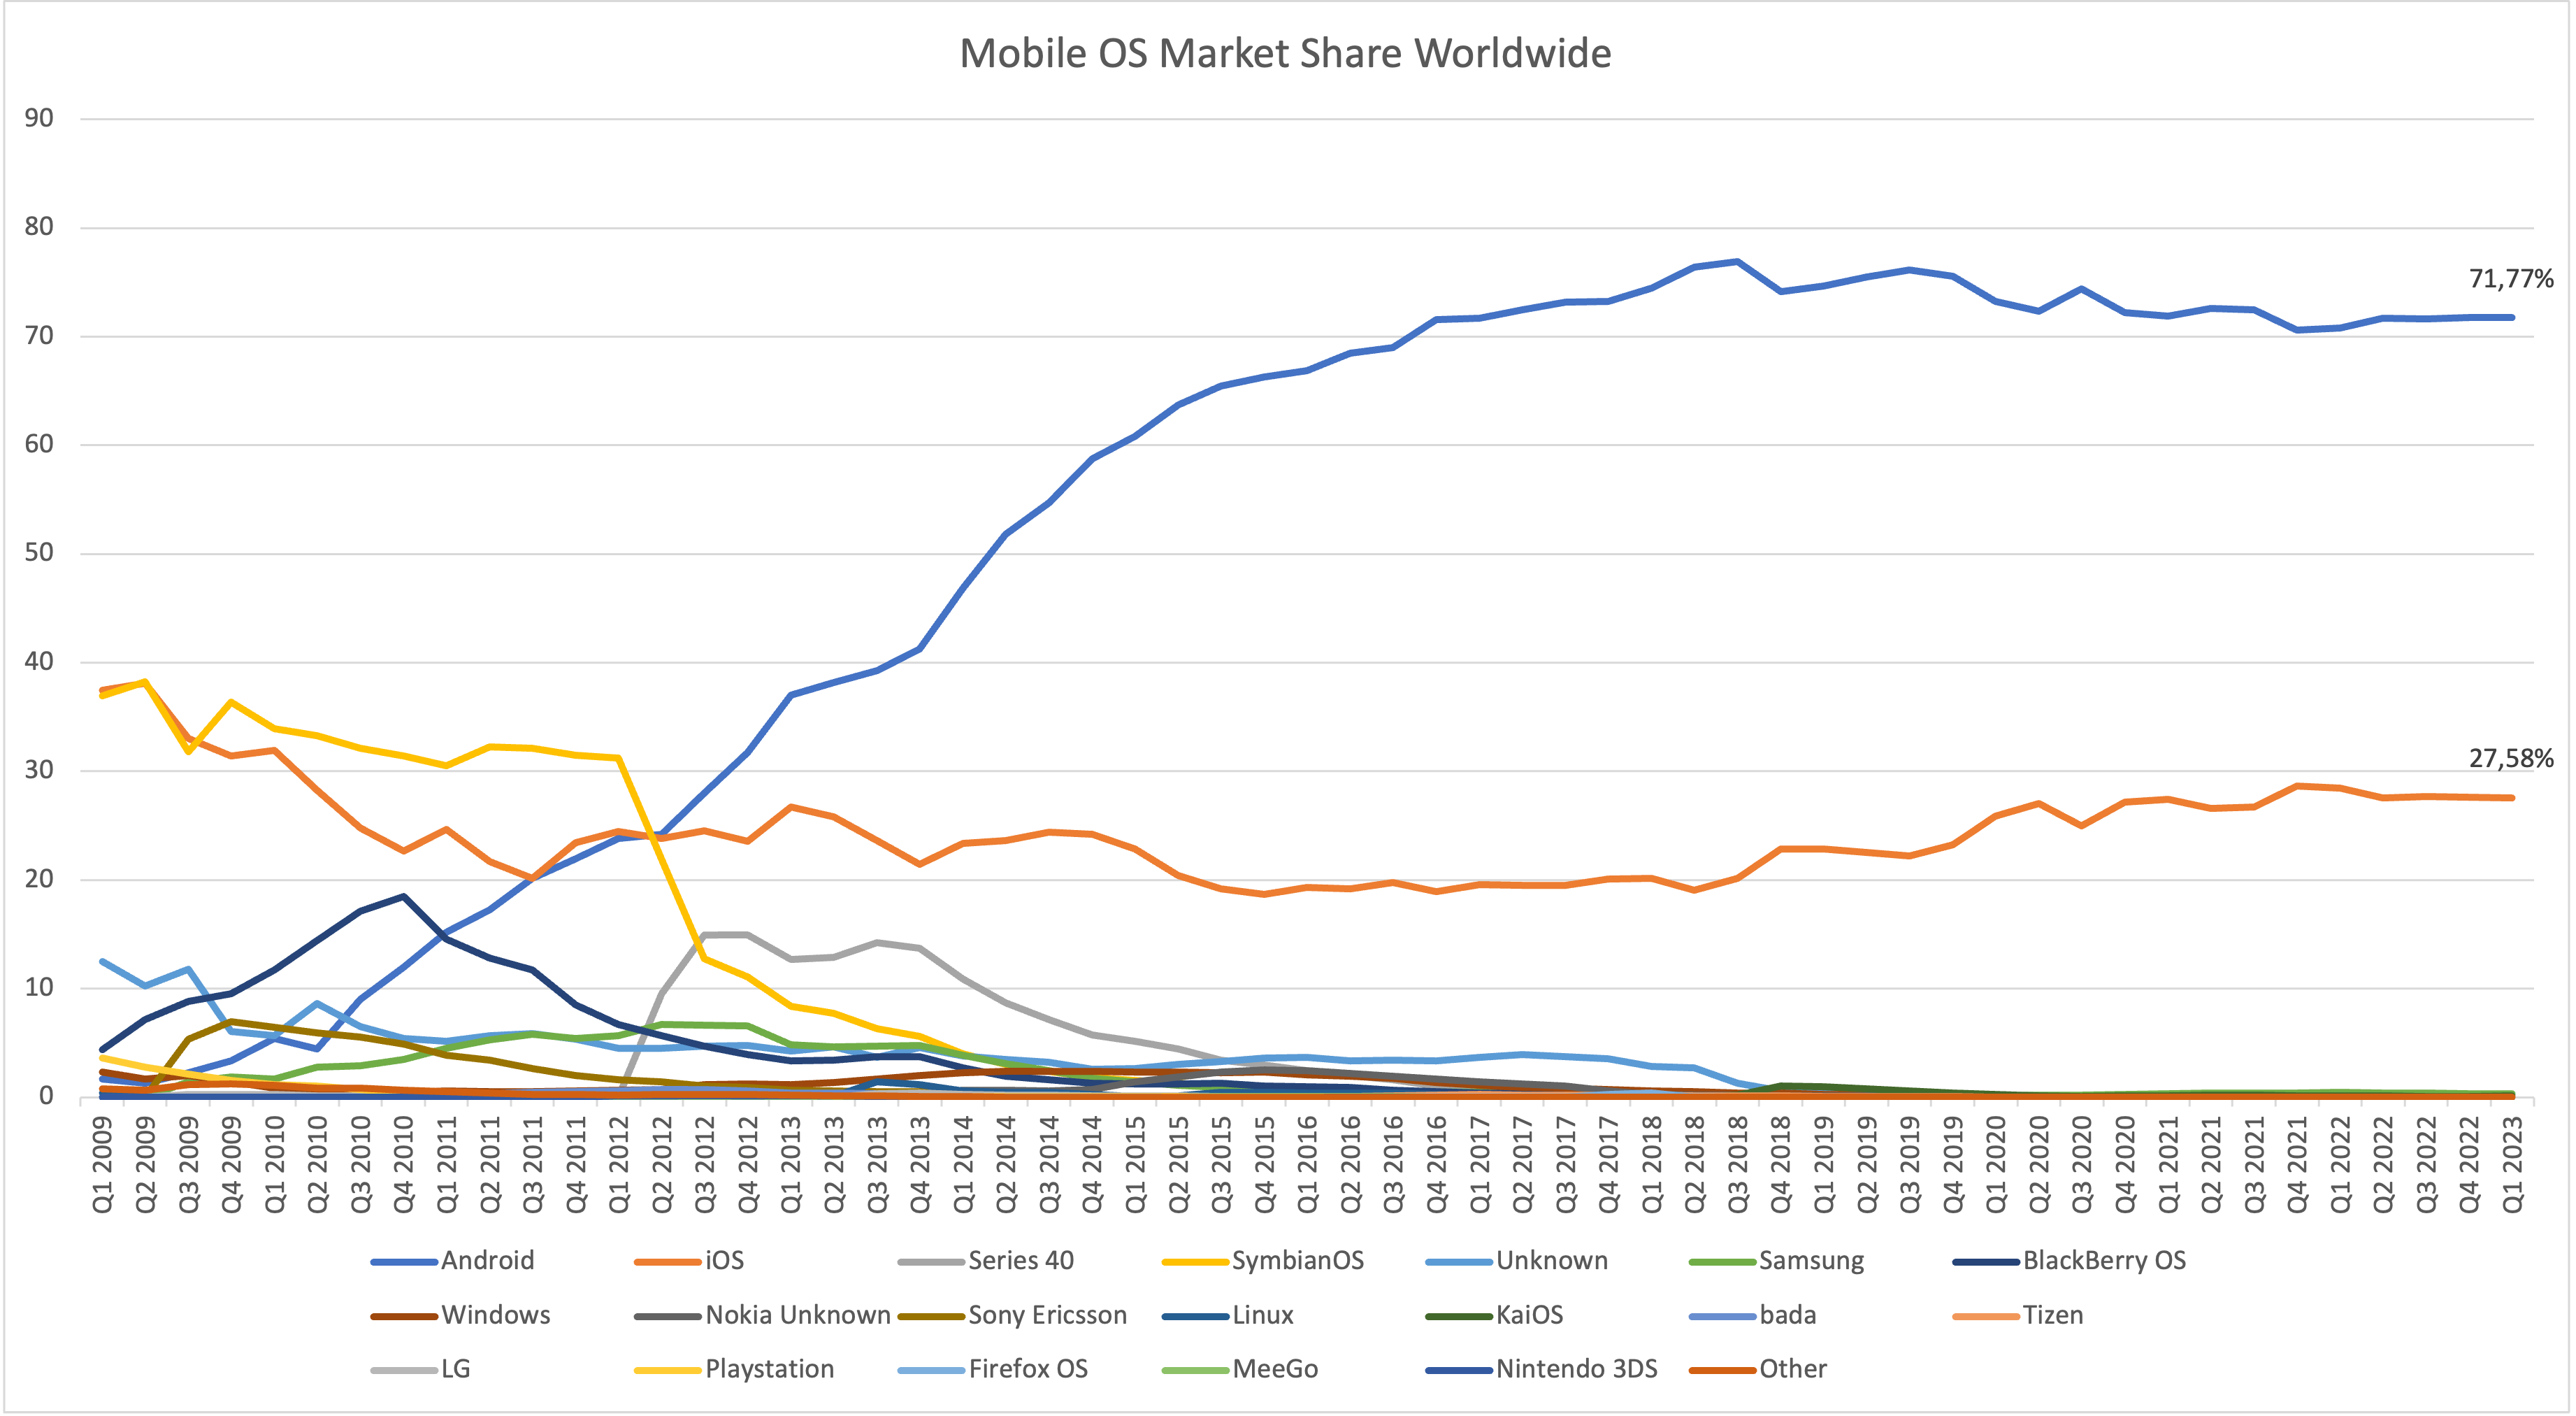
\includegraphics[width=\textwidth]{img/mobile_os_market}
  \caption{Mobile OS market (Source: Own work based on \cite{statcounter_mobile_os_market})}
  \label{fig:mobile_os_market}
\end{figure}

As can be seen in the Figure \ref{fig:ios_versions}, in case of iOS, almost 90\% of devices are running either the most or second-most recent major version of the operating system. Therefore, when targeting the Apple's system, probably a single codebase would be enough to guarantee the appropriate coverage.

However, in case of Android, there is a high level of market fragmentation, as nearly 20\% of smartphones or tablets are running older versions released as far as in 2015 (Figure \ref{fig:android_versions}). Because there are limitations such as deprecation of code commands and API (Application Programming Interfaces) behavior changes between distant versions, multiple codebases may be chosen to be maintained separately per a single mobile application. Another issue is the fact, that device manufacturers are able to apply various modifications to the operating system which can lead to errors occurring only on those devices \cite{comparison_technologies_multiplatform}, causing difficulties for developers. Because Apple is the exclusive manufacturer of devices running iOS, they do not suffer from such a problem. 

\begin{figure}[ht]
  \begin{minipage}{.47\textwidth}
    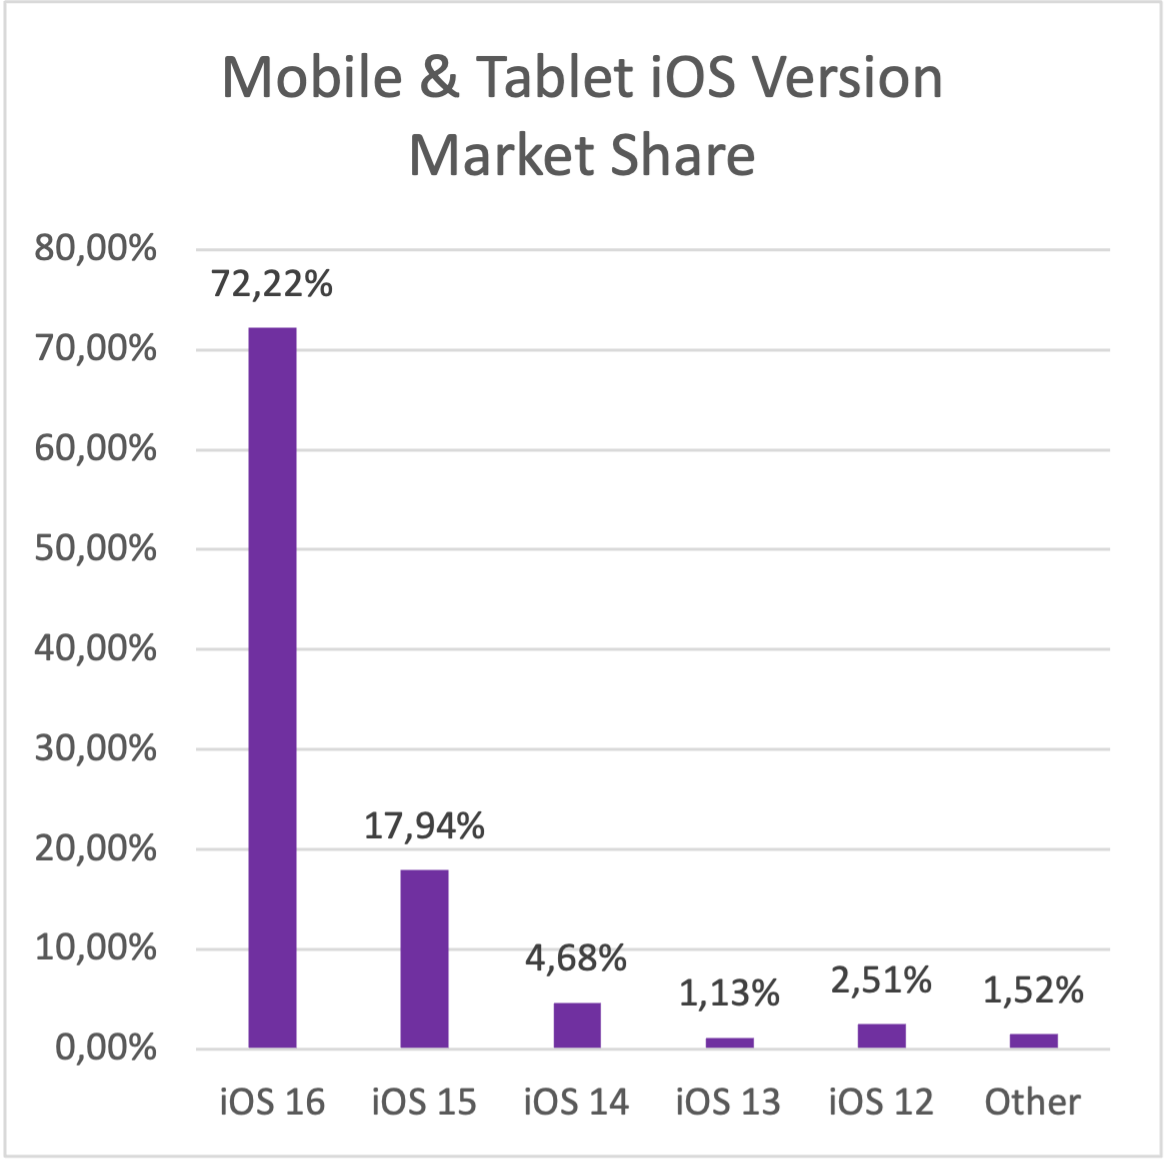
\includegraphics[width=\textwidth]{img/ios_ver_market_share}
    \caption{iOS version market share (Source: Own work based on \cite{statcounter_ios_version_market})}
    \label{fig:ios_versions}
  \end{minipage}
  \hfill
  \begin{minipage}{.47\textwidth}
    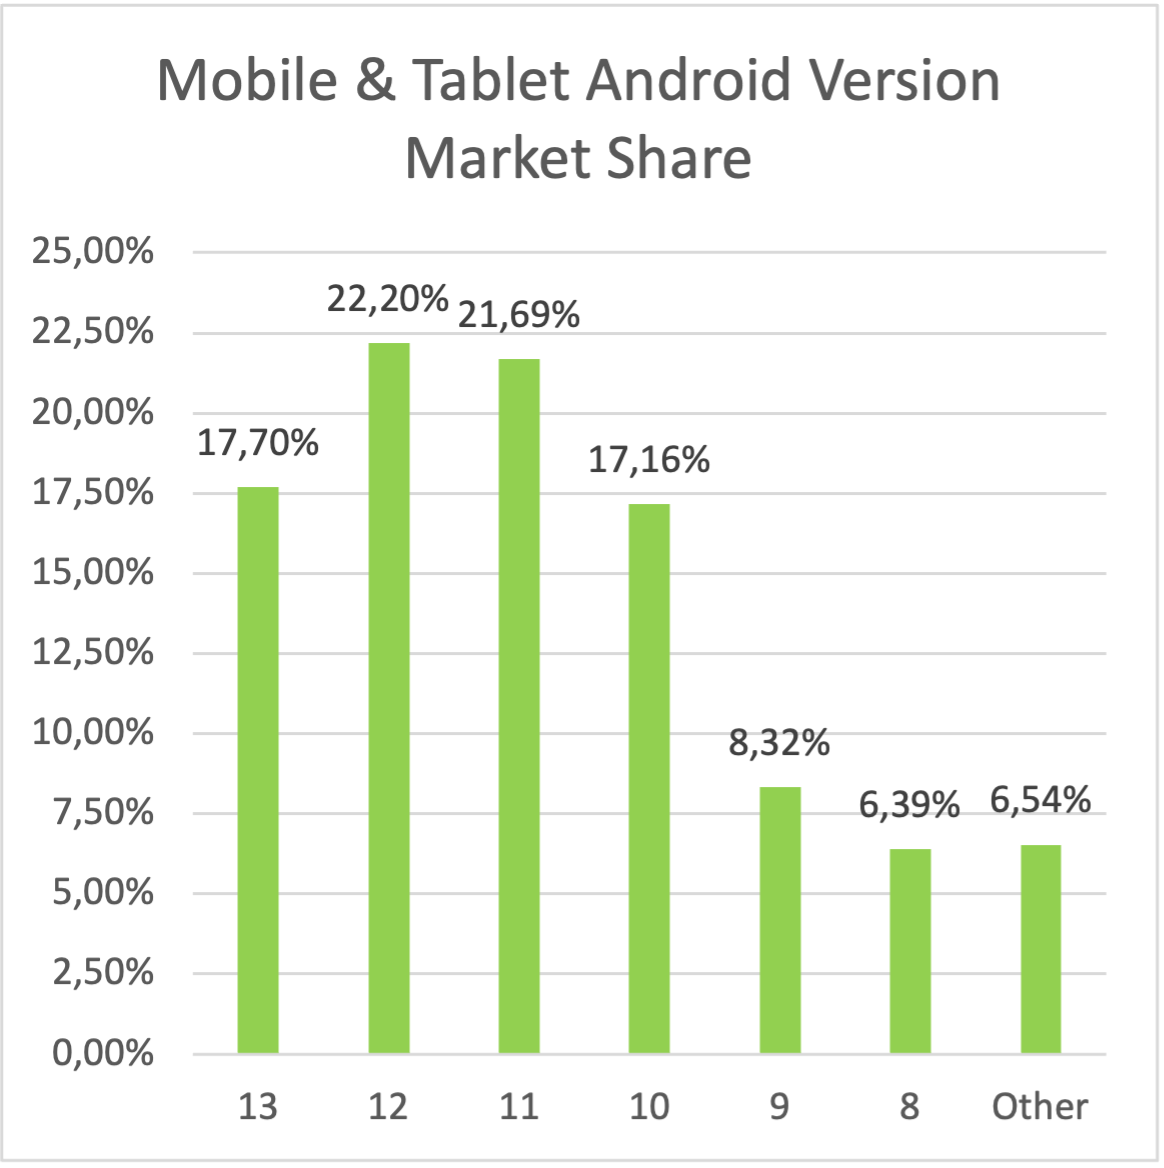
\includegraphics[width=\textwidth]{img/android_ver_market_share}
    \caption{Android version market share (Source: Own work based on \cite{statcounter_android_version_market})}
    \label{fig:android_versions}
  \end{minipage}
\end{figure}

\subsubsection{Android}

Android is an open-source operating system developed by the Open Handset Alliance and Google to run mainly on mobile devices such as smartphones and tablets but also TVs and cars \cite{android_what_is,comparison_technologies_multiplatform}. It is based on the Linux kernel and has a multiple-component structure \cite{android_architecture_and_application}, as can be seen in the Figure \ref{fig:android_architecture}. Each part takes responsibility for different tasks, e.g., Android Runtime provides optimized garbage collection and View System (included in Java API Framework) enables developers to implement the user interface layouts using various elements such as lists and buttons \cite{android_architecture}.

\begin{figure}[h]
    \centering
    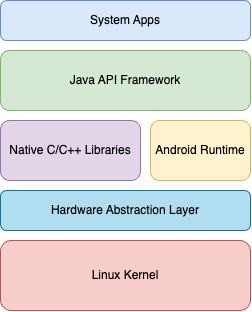
\includegraphics[scale=0.73]{img/android_architecture}
    \caption{Android architecture (Source: Own work based on \cite{android_architecture})}
    \label{fig:android_architecture}
\end{figure}

It is not necessary to use an IDEs (Integrated Development Environment) to build most software. Despite that, most programmers tend to reach out to them because of the guaranteed development comfort and productivity increase. Android Studio is the primary IDE for native mobile development of Android applications. It is created on top of IntelliJ's IDEA and provides numerous features such as Gradle, advanced debugging tools and profilers, etc \cite{android_studio_intro}.

For many years, Java has been the official language for Android development. However, since Google established Kotlin as the default choice in 2019 \cite{android_kotlin_first}, over 60\% of programmers have switched to it \cite{android_kotlin}. Furthermore, data shows that almost 90\% of the Google Play Store Top 500 USA mobile apps have been developed with it \cite{kc_kotlin_vs_java}. Kotlin's popularity is certainly going to grow in the upcoming years, considering the undeniable benefits it brings. Still, there are some scenarios in which Java could remain the first choice.

Table \ref{tab:java_kotlin_comparison} shows that all the features necessary for Android application development, such as e.g., Android SDK or AndroidX support, are fully provided by both Java and Kotlin. Furthermore, the latter introduces additional advantages in the form of enabling the usage of Jetpack Compose toolkit and even the ability to create multi-platform projects (Kotlin Multiplatform is currently only accessible in Beta version \cite{kotlin_multiplatform}).

\begin{table}[h]
  \centering
    \caption{Java and Kotlin comparison (Source: Own work based on \cite{android_kotlin_first})}
    \label{tab:java_kotlin_comparison}
    \begin{tabular}{ | p{55mm} | >{\centering}p{33mm} | >{\centering\arraybackslash}p{33mm} | }
      \hline
      \multicolumn{1}{ |c| }{\textbf{Feature}}&\textbf{Java}&\textbf{Kotlin}\\
      \hline
      Platform SDK support&Yes&Yes\\
      \hline
      Android Studio support&Yes&Yes\\
      \hline
      Lint&Yes&Yes\\
      \hline
      Guided docs support&Yes&Yes\\
      \hline
      API docs support&Yes&Yes\\
      \hline
      AndroidX support&Yes&Yes\\
      \hline
      AndroidX Kotlin-specific APIs (KTX, croutines, \dots)&N/A&Yes\\
      \hline
      Online training&Best effort&Yes\\
      \hline
      Samples&Best effort&Yes\\
      \hline
      Multi-platform projects&No&Yes\\
      \hline
      Jetpack Compose&No&Yes\\
      \hline
      Compiler plugin support&No&Yes (Kotlin Symbol Processing API)\\
      \hline
    \end{tabular}
\end{table}

Java is a high-level object-oriented programming language introduced as far back as 1995. It is one of the most popular languages in the world which is regularly updated, reaching major version 20 this year. However, in the context of Android development the supported versions are 8 and 11, with the latter requiring high Android API version in order to use all the offered elements (although upgraded API desugaring announced in February this year broadens the range of libraries available without increasing the app's minimum supported API level \cite{android_api_desugaring}). The advantages of Java mainly result from the fact it is present for a very long time. During the last 30 years it gathered a big community of developers with high-level experience. Therefore, it may be easier to form a competent team for the project. Moreover, there are numerous applications that had been created with Java which owners might not seek for a migration, which as a result maintains Java's importance in the market \cite{kc_kotlin_vs_java}.

On the other hand, Kotlin offers many assets because of which it has replaced Java as an official first-choice language for Android development, as mentioned before. Kotlin is a comparatively recent programming language introduced in 2016 by JetBrains. First and foremost, it is fully interoperable with Java and therefore, it is possible to call Kotlin code inside Java code and vice versa. Secondly, Kotlin's syntax is very concise and null-safe, thus increasing the speed of development and reducing the project's code lines and lowering the possibility of mistakes. For those reasons, implementation of new apps using Kotlin is fairly straight-forward and comfortable from the point of view of developers. Moreover, the migration of existing projects from Java to Kotlin is uncomplicated and can lead to size decrease and simplification of the codebase with much smaller Null Pointer Exception occurrence in runtime \cite{android_kotlin_first}.

Since Kotlin has already been established as the preferred programming language for Android development, all considerations in the scope of this thesis will be limited to it rather than Java.

One of the possibilities acquired when selecting Kotlin for Android development is the ability to use Jetpack Compose. It is a powerful toolkit used for building User Interface layouts introduced in 2021 with a goal improve that process compared to the previous XML approach \cite{android_jetpack_compose}. 
The main difference between the above-mentioned methods is the fact that they represent declarative and imperative approach, respectively. The former greatly reduces the amount of boilerplate code improving readibility as well as build time and therefore, increases development efficiency. Additionally, just as Kotlin offers interoperability with Java, Jetpack Compose provides the same in regards to XML. In short, XML approach implies the creation of layouts in XML markup files and later referencing them in the code while implementing the behavior. On the other hand, Jetpack Compose makes use of prebuilt components and intuitive state management \cite{jetpack_compose_vs_xml}. 

In order to improve the user experience accross different apps, Material design system was introduced by Google in 2014. First versions were strictly connected to Android only, however since then it has shifted towards being applicable for other platforms, including Web. Material provides detailed guidelines in the aspect of styling, accessibility, overall UX as well as prebuilt reusable UI components aiming to improve the efficiency of developing apps that are intuitive and responsive. The main principles are that every element of an app should be considered as a physical material and they should be combined together in layers while putting emphasis on natural animations and universal clarity. The big advantage of Material being applied in mobile apps is the fact that when a user understands how to use one it is automatically transposed onto others. On the other hand, an issue may be raised that if all the mobile apps available conformed to one design system, they would become overly monothematic and characterless \cite{material_design_get_started,material_design_pros_cons}.

\subsubsection{iOS}

iOS is the Apple's closed-source operating system based on Darwin OS that runs exclusively on Apple's smartphones (iPhones). It also lays beneath other mobile systems: iPadOS, tvOS and watchOS. It includes four layers that together enable the interaction between hardware and applications, as presented in Figure \ref{fig:ios_architecture}. Core OS layer provides necessary low-level services, e.g. Bluetooth, security and 64-bit support. Core Services layer incorporates multiple interfaces called Frameworks which are responsible for functionalities such as data management, cloud transfer and location. Media layer's task is to handle graphics and audio technology. Finally, Cocoa Touch enables user-application interaction, mainly through the implementation of touch gestures \cite{ios_architecture,mobile_os_survey}.

\begin{figure}[h]
  \centering
  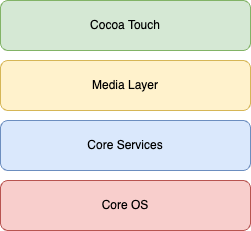
\includegraphics[scale=0.73]{img/ios_architecture}
  \caption{iOS architecture (Source: Own work based on \cite{ios_architecture})}
  \label{fig:ios_architecture}
\end{figure}

Xcode is the primary IDE for building iOS, iPadOS, watchOS, tvOS and macOS applications. It offers tools necessary for the whole range of development: implementation, testing, optimization and deployment. It includes Developer Tools, e.g. Simulator for testing, Instruments for performance profiling and Reality Composer for 3D and AR features \cite{xcode_documentation}. Native iOS development comes with additional costs compared to Android because Xcode requires a Mac device, e.g. the MacBook laptop, which itself can be expensive especially when considering a large development team \cite{comparison_technologies_multiplatform,comp_study_hybrid}.

Currently, the officially recommended programming language for iOS development is Swift. It was introduced with the goal to replace previously used Objective-C. Essentially, it was supposed to increase the ease of development and maintenance of the codebase, make it more error-proof and performant. Objective-C remains supported by Apple for the indefinite future, however since 2011, it has not received any major updates staying at version 2.0 \cite{swift_overview,speed_performance_swift_objective_c,swift_vs_objective_c,wiki_objective_c}.

Objective-C is an object-oriented, dynamically-typed programming language published in 1984. Similarly to Java for Android development, Objective-C is very stable because of its age and is still necessary for legacy applications support because Swift does not allow development of applications for lower than 7.0 version of iOS. Additionally, it allows Swift code usage by automatically regenerating files to enable the integration, which makes it possible to keep the existing code in old projects even when migrating to Swift \cite{swift_objective_c_new_language,geeks_objective_c_swift}.

Swift is a compiled, statically-typed programming language introduced by Apple in 2014. It holds the features of Objective-C while providing various improvements such as automatic memory management (ARC). Its syntax is much more concise, resulting in readable and easily maintainable code, as well as quicker development time. It was emphasized on release that Swift increases safety and it does so by overflow checking, optionals, type safety, etc. Furthermore, Swift has been shown to run faster than Objective-C. It is also fully interoperable with Objective-C code \cite{swift_overview,swift_objective_c_new_language,geeks_objective_c_swift}. However, one of the issues is differences between iOS versions that may force code rewriting. Finally, an important advantage of Swift is that it enables the usage of SwiftUI \cite{comparison_technologies_multiplatform}.

In iOS development, there are multiple ways to implement user interface views. Apple offers two design solutions which can be used together if needed: UIKit and the more recent SwiftUI. The latter has been acknowledged by Apple to be the primary solution \cite{comparison_technologies_multiplatform}. UIKit is an imperative framework that can be applied programmatically (imperatively) or by using Interface Builder to create XIBs (XML Interface Builder) or Storyboards, while SwiftUI is a declarative framework. The difference in programming paradigms results in less code lines necessary for the same task when programming with SwiftUI. Furthermore, SwiftUI apps can be built for all platforms of Apple devices, while UIKit is meant only for iOS, iPadOS and tvOS and requires AppKit and WatchKit to support the rest. On the other hand, SwiftUI supports iOS version 13.0 minimum so if further backwards compatibility is needed than UIKit remains the first choice \cite{swiftui_overview,xib_why_use,swiftui_uikit}.

In order to provide consistency among different applications and across different Apple platforms, Human Interface Guidelines (HIG) has been introduced. It is a document containing detailed general and platform-specific design principles and practices. Developing applications according to that information helps guarantee that the end product is in accordance with Apple's standard, both visually and behaviorally. Consequently, great user experience is reached as users can easily comprehend applications that are similar and consistent with the platform they are used to, e.g. the positioning of action buttons and touch gestures in iOS apps. Exemplary aspects underlined in HIG are layout creation, navigation, inputs, accessibility, technology support and more \cite{hig_overview}.

\subsubsection{Web development in relation to native mobile development}

While solely native mobile development has been considered in this chapter, it is important to reflect upon its connection to web development. Of course, it is a possibility that a service is designed to be available exclusively in the form of a mobile application and such attitude will remain unchanged in the future. However, there are some reasons for which a publisher may look to extend the supported platform list after time. For instance, a small service may start as an Android application and grow enough to need other platforms in order to reach a bigger volume of users. In such a case, iOS support may be added as well as a website may be developed. The second option is especially probable as it provides accessibility for all platforms. The fact that such a service launched in the shape of a single-platform application in the first place may be caused by many aspects, such as dictated functional requirements, detachment or overlook during the initial planning stages as well as market trends analysis \cite{web_mobile_app}. Cross-platform frameworks could be the answer to the above-mentioned issues.
